\documentclass[t,xcolor={usenames,dvipsnames}]{beamer}

\mode<presentation>
{
\usetheme{Warsaw}
}


\usepackage[english]{babel}
\usepackage[latin1]{inputenc}
\usepackage{times}
\usepackage[T1]{fontenc}
\usepackage{hyperref}



% Where \includegraphics should look for figures
\graphicspath{{./figs/}}
\usepackage{epstopdf}
\DeclareGraphicsExtensions{.eps,.png,.jpg,.pdf}

% Useful shortcuts / styling
\newcommand{\myhref}[2]{\href{#1}{\textcolor{Blue}{#2}}}
\newcommand{\doi}[1]{\myhref{http://dx.doi.org/#1}{doi:#1}}
\newcommand{\subitem}[1]{\begin{itemize}[<.->]\item #1 \end{itemize}}
\newcommand{\csym}[1]{\textcolor{Blue}{\texttt{#1}}}

%%%%%%%%%%%%%%%%%%%%%%%%%%%%%%%%%%%%%%%%%%%%%%%%%%%%%%%%%%%%%%%%%%%%%%
% Title, author, logo
\title{Functional Curation: Potential Future Directions for SED-ML}
\author[Jonathan Cooper]{Jonathan Cooper \and Gary Mirams}
\institute[University of Oxford]
{Computational Biology Group\\
 Department of Computer Science\\
 University of Oxford}
\date{3\textsuperscript{rd} September 2011}

\begin{document}

\begin{frame}
\titlepage
\note{Some colleagues and I have been creating a system to provide what we're calling Functional Curation.  In doing so we've developed several ideas that we think will be of benefit to include in future levels of SED-ML, to enhance the capabilities of the language greatly, with relatively little extra effort in implementation.}
\end{frame}

\begin{frame}{Outline}
\tableofcontents
\note{I'll start by explaining what Functional Curation is, and its requirements that influence our proposals.  I'll then discuss the main proposals themselves.  There are far more technical details than can be included in a talk of this nature, so I'll focus on explaining the high-level concepts and why they're useful; a technical review of specific proposals of interest to the community can follow later.  My final slide will enumerate all the proposals briefly as an aid to discussion.}
\end{frame}


%%%%%%%%%%%%%%%%%%%%%%%%%%%%%%%%%%%%%%%%%%%%%%%%%%%%%%%%%%%%%%%%%%%%%%
\section{Introduction to Functional Curation}

\begin{frame}{Functional Curation}
\note{Only rarely will you have a single model of any particular system.  We have incomplete knowledge, and develop models to explore and compare hypotheses.}
\begin{itemize}
\item How can we compare models?
\item Which model is best suited to investigating this experiment?
\item What functionality does a model have?
\end{itemize}
We are implementing a system to answer these questions.
\end{frame}

\begin{frame}{Using protocols}
\begin{itemize}[<+->]
\item A \alert{protocol} is the \textit{in silico} version of an experiment, that can be applied to models of the system in question
\item A \alert{language} is needed to describe protocols
  \subitem{SED-ML?}
\item In SED-ML, a protocol specifies the model
\item We want one protocol, \alert{many} models
\item One model, many protocols
\item Many models, many protocols
  \note<.>{Characterise a whole repository}
\end{itemize}
\end{frame}

\begin{frame}{Complex post-processing}
\note{Often the raw simulation results will not be of primary interest.  Recognising this, SED-ML has support for post-processing, but\ldots}
\begin{itemize}
\item SED-ML \texttt{dataGenerator}s are currently fairly restrictive
\item Many standard cardiac protocols require additional functionality
\item Example: S1-S2 restitution
\end{itemize}
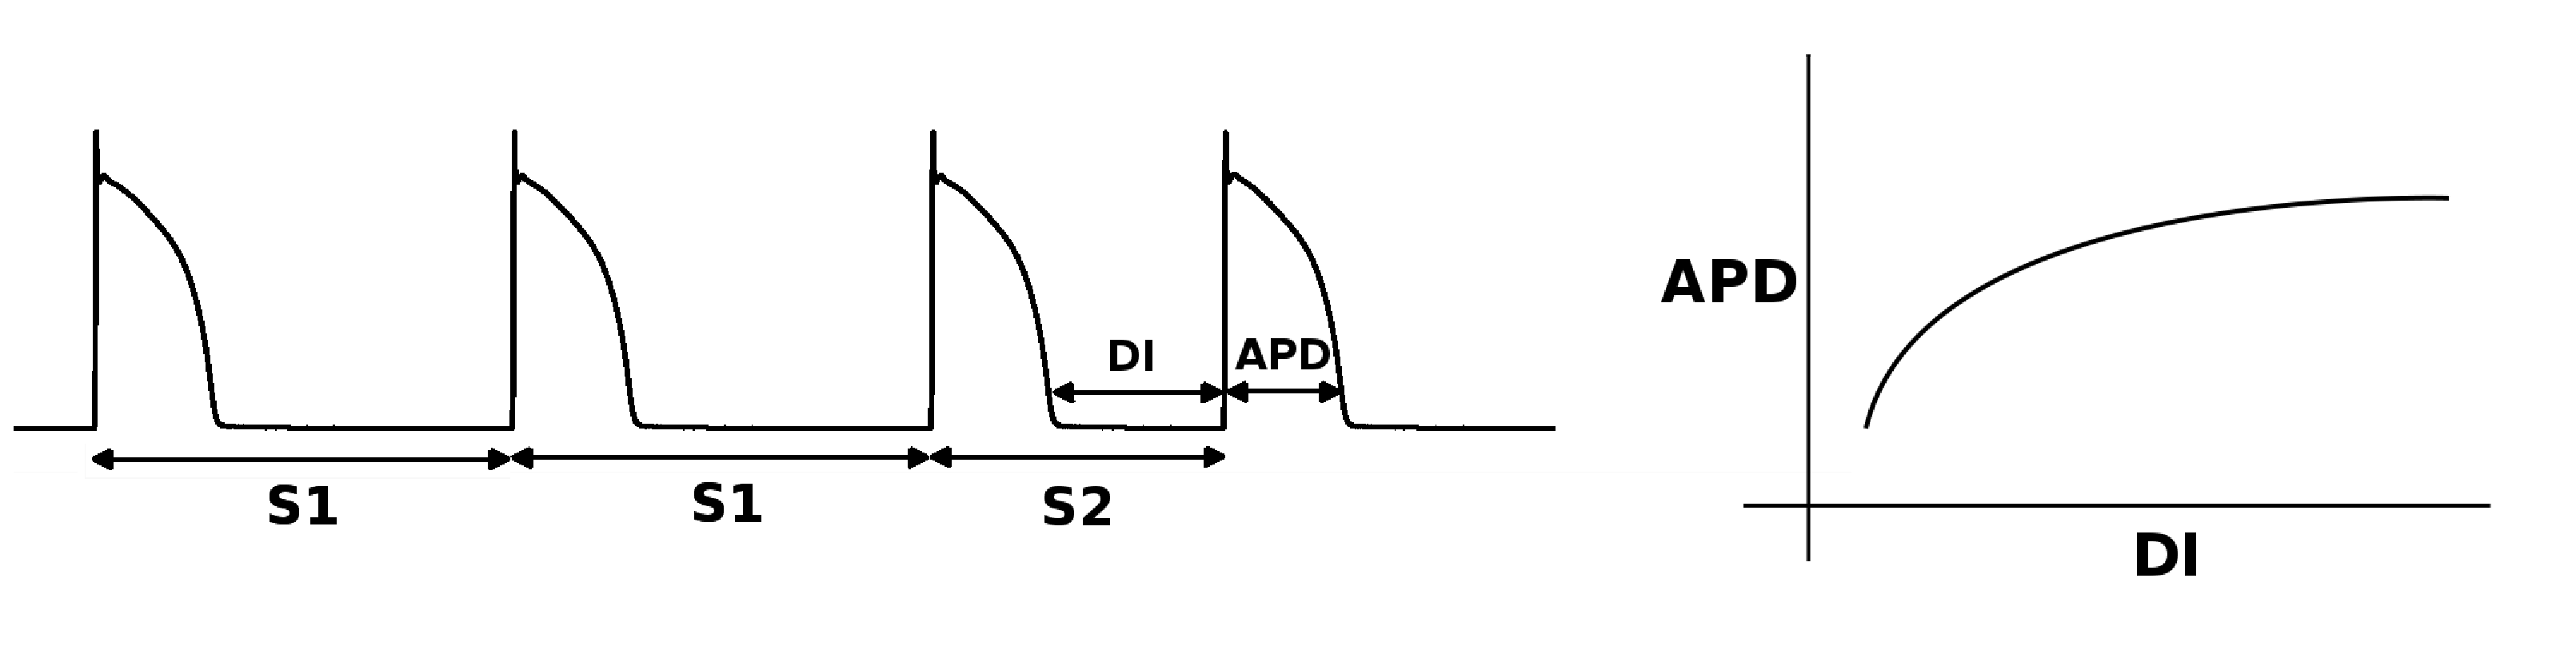
\includegraphics[width=\textwidth]{S1S2}
\end{frame}

\begin{frame}{Example: S1-S2 protocol on canine models}
\note{As part of our system to run protocols such as this, we're building our own prototype protocol language, to investigate ideas and see what works, what's needed to provide the necessary functionality.}
Our system currently has its own protocol language.
We'd like to use SED-ML instead!
\vspace{-.6cm}
\begin{columns}[T]
\begin{column}{.33\linewidth}
\begin{center}
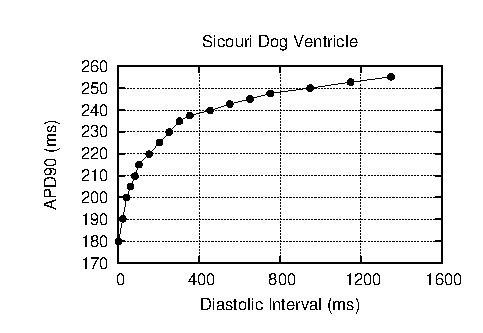
\includegraphics[width=\textwidth]{sicouri_dog_ventricle_s1s2_curve}\\
\vspace{.1cm}
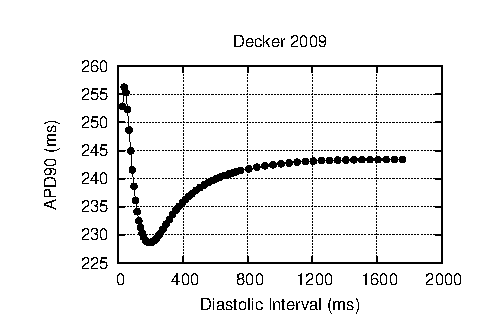
\includegraphics[width=\textwidth]{decker_2009_s1s2_curve}
\end{center}
\end{column}
\begin{column}{.33\linewidth}
\begin{center}
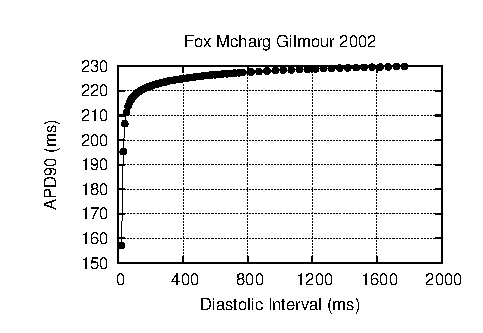
\includegraphics[width=\textwidth]{fox_mcharg_gilmour_2002_s1s2_curve}\\
\vspace{.1cm}
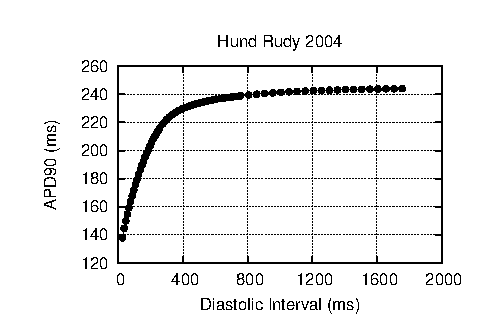
\includegraphics[width=\textwidth]{hund_rudy_2004_s1s2_curve}
\end{center}
\end{column}
\begin{column}{.33\linewidth}
\begin{center}
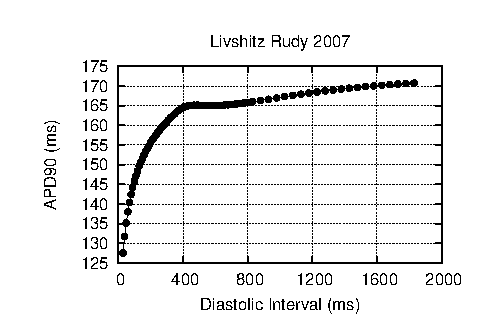
\includegraphics[width=\textwidth]{livshitz_rudy_2007_s1s2_curve}\\
\vspace{.1cm}
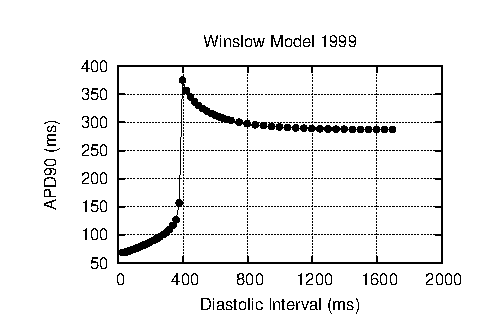
\includegraphics[width=\textwidth]{winslow_model_1999_s1s2_curve}
\end{center}
\end{column}
\end{columns}
\vspace{.3cm}
\scriptsize{See also \doi{10.1016/j.pbiomolbio.2011.06.003}}
\end{frame}


%%%%%%%%%%%%%%%%%%%%%%%%%%%%%%%%%%%%%%%%%%%%%%%%%%%%%%%%%%%%%%%%%%%%%%
\section{Suggestions for SED-ML}


\begin{frame}{Suggested extensions to SED-ML}
These are features our protocol language has, that we would like to see added to SED-ML, in order to represent a wider range of experiments.
\begin{itemize}[<+->]
\item Interfacing protocols with models
  \subitem{Ontologies, units, model inputs and outputs}
\item Sequenced and nested simulations
  \subitem{Based on Frank Bergmann's proposal}
\item $N$-dimensional array based post-processing
  \subitem{Minimal extensions to MathML, many possibilities}
\item Protocol libraries for usability
  \subitem{Allow different UIs to target different levels of user}
\end{itemize}
\end{frame}

\begin{frame}{The parts of our protocols}
\note{The talk will focus on the highlighted aspects which are most relevant to the proposals just mentioned.  However, it's worth putting them in context.}
\begin{itemize}
\item Documentation
\item Input specifications
\item Protocol imports\footnote{\tiny Not yet implemented}
\item Library definitions
  \note{Functions \& variables for later use}
\item Units definitions
  \note{Currently using CellML's elements}
\item<alert@1> Model interface
\item<alert@1> Simulations
\item<alert@1> Post-processing
\item Output specifications
  \note{What isn't just an intermediate result}
\item Plot specifications
\end{itemize}
\end{frame}

%%%%%%%%%%%%%%%%%%%%%%%%%%%%%%%%%%%%%%%%%%%%%%%%%%%%%%%%%%%%
\subsection{Interfacing protocols and models}

\begin{frame}{Referring to model variables}
\begin{itemize}
\item SED-ML uses XPath to locate variable elements
\item What if models use different naming conventions or structures?
\item Instead, use \alert{ontological annotation} of variables
\item Protocol can use \texttt{prefix:name} notation as for XML namespaces
\item No need for `approved' ontology --- just need model \& protocol to agree
\end{itemize}
\end{frame}

\begin{frame}{Units conversions}
\begin{itemize}
\item Different models use different units
\item Protocol declares the units it uses, and conversions applied automatically
  \note{This is easy for scalings within a dimension, but models can use different approaches to representing the same biology, e.g.\ different normalisation for ionic currents}
\item ``Biology-aware'' conversion rules can be defined
  \begin{itemize}
  \item A unary function for converting a value from one dimension to another
  \item Can refer to model variables using ontology terms
  \item Fall-back to next rule if required variables don't exist
  \item See also \doi{10.1016/j.pbiomolbio.2011.06.002}
  \end{itemize}
\end{itemize}
\end{frame}

\begin{frame}{Model modifications}
\begin{itemize}
\item Abstraction of SED-ML \texttt{Change} functionality
\item A model is viewed as a \alert{system of equations}, independent of modelling language
\item<2-> Protocol specifies which variables are \alert{inputs} and \alert{outputs}
\item<2-> Inputs become parameters that can be set by the protocol
  \subitem{e.g. voltage clamp experiment}
\item<2-> Only those equations required for the given outputs need be computed
\item<3-> Equations may also be \alert{added or replaced}
  \subitem{e.g. to specify a stimulus current waveform}
\end{itemize}
\end{frame}

%%%%%%%%%%%%%%%%%%%%%%%%%%%%%%%%%%%%%%%%%%%%%%%%%%%%%%%%%%%%
\subsection{Sequenced and nested simulations}

\begin{frame}{Sequenced and nested simulations}
\begin{itemize}[<+->]
\item An experiment may have `setup' and `measurement' phases $\implies$ simulations should be able to run in sequence
  \subitem{Simulations may define a prefix, allowing outputs from any simulation in a sequence to be addressed}
\item Nesting simulations supports parameter scans, repeated runs, distribution sampling, etc.
  \subitem{\alert{Model outputs therefore become regular $n$-dimensional arrays}}
\end{itemize}
\end{frame}

\begin{frame}{Modifiers}
\begin{itemize}
\item Each simulation can have a collection of \alert{modifiers}
  \begin{itemize}
  \item There are 3 kinds of modifier:
    \begin{description}
    \item[SaveState] store the current model state, giving it a name
    \item[ResetState] reset the model to a stored state or initial conditions
    \item[SetVariable] set the value of a model variable\\
      The value is given by an expression in the post-processing language,
      and can access the current range value for this or any outer loop.
    \end{description}
  \item Each can be applied just at the start or end of a simulation, or prior to each loop
  \end{itemize}
\end{itemize}
\end{frame}

%%%%%%%%%%%%%%%%%%%%%%%%%%%%%%%%%%%%%%%%%%%%%%%%%%%%%%%%%%%%
\subsection{Post-processing}

\begin{frame}{Post-processing language}
\begin{itemize}
\item Aim to support complex operations with minimal implementation overhead
\item Therefore base on MathML, with as few as possible added \csym{csymbol}s
\item Key features:
  \begin{itemize}
  \item Operators for working with $n$-dimensional arrays
  \item Sequencing operations (assignments to variables, assertions)
  \item Defining functions (that can also be passed to other functions)
  \end{itemize}
\item Not just used for post-processing: also input specifications, library definitions, etc.
\item Technically, this is a pure functional $n$-dimensional array based programming language
\end{itemize}
\end{frame}

\begin{frame}{Main special expressions}
\footnotesize
\begin{description}
\item[\csym{newArray}] Create a new array
  \begin{itemize}
  \item by listing elements (which may be arrays)
  \item by \alert{comprehension} using a generator expression with index ranges
  (abusing \texttt{domainofapplication})
  \end{itemize}
\item[\csym{view}] Extract a sub-array
  \subitem{Can use arbitrary (even negative) strides over any dimension, with wildcards}
\item[\csym{map}] Map an $n$-ary function onto $n$ arrays element-wise
\item[\csym{fold}] Collapse an array along a single dimension using a binary function
  \subitem{Used to define \texttt{sum}, \texttt{max}, etc.}
\item[\csym{find}] Find indices where the operand array is non-zero
\item[\csym{index}] Create a sub-array containing only the given indices
  \subitem{Various options for avoiding irregular results}
\end{description}
\end{frame}

%%%%%%%%%%%%%%%%%%%%%%%%%%%%%%%%%%%%%%%%%%%%%%%%%%%%%%%%%%%%%%%%%%%%%%
\section{Summary}

\begin{frame}{Summary of proposals}
\begin{itemize}
\item Interfacing protocols with models
  \begin{itemize}
  \item Refer to model variables with ontology terms
  \item Apply units conversions, with user-defined rules
  \item Modify model equations if required/possible
  \end{itemize}
\item Sequenced and nested simulations
  \begin{itemize}
  \item Hence outputs are $n$-dimensional arrays
  \item Vector ranges using post-processing language to compute $1$d array
  \item Modifers: save/load model state, set variable
  \end{itemize}
\item Array-based post-processing
  \begin{itemize}
  \item Functions can be defined in the language
  \item Operations can be sequenced
  \item Array comprehensions, views, map, fold, find \& index
  \end{itemize}
\item Protocol libraries for usability
\end{itemize}
\note{Finish with sales pitch: can do more with SED-ML, get more users!}
\end{frame}


%%%%%%%%%%%%%%%%%%%%%%%%%%%%%%%%%%%%%%%%%%%%%%%%%%%%%%%%%%%%%%%%%%%%%%
\appendix

\begin{frame}{Extra slides}
The slides that follow are not central to the talk, but have extra bits
of information that might be useful for questions.
\end{frame}

\begin{frame}{Ranges}
\note{This slide could be cut as there's very little novelty.}
\begin{itemize}
\item Each simulation requires a \alert{range} over which to iterate for generating output points
  \begin{itemize}
  \item \texttt{UniformRange}, \texttt{VectorRange} and \texttt{FunctionalRange} have been proposed
  \item Using post-processing language constructs to define an array of values, our \texttt{VectorRange} can implement all of these
  \note{Although we still have \texttt{UniformRange} too, as the simple case arises often}
  \end{itemize}
\end{itemize}
\end{frame}

\begin{frame}{Nested protocols}{\tiny (Not yet implemented)}
\begin{itemize}
\item Since a protocol has inputs and outputs, it can be viewed as a kind of model
\item The ``system of equations'' abstraction does not apply, so model modifications are not possible
\item This does effectively allow us to interleave post-processing and simulation however
\item So we can do e.g.\ dynamic restitution without breaking the `regular $n$-d array' data model
\end{itemize}
\end{frame}

\begin{frame}{Environments}
\begin{itemize}
\item A store mapping names to values
\item Bindings may not be overwritten
\item Multiple environments exist
  \subitem{e.g.\ for protocol inputs, library, model variables, simulation ranges \& outputs, post-processing operations \& results, function locals}
\item Environments can delegate lookups
  \begin{itemize}
  \item Prefixed references go to the associated environment (e.g.\ specific simulation, imported protocol, model variable)
  \item Many also have a default delegatee
  \end{itemize}
\end{itemize}
\end{frame}

\begin{frame}{Statements}
\begin{itemize}
\item The \csym{statementList} is used for function bodies, and the library \& post-processing sections
\item 3 kinds of statement:
  \begin{itemize}
  \item Assignment: MathML \texttt{eq}
  \item Return: \csym{return} --- only valid in functions
  \item Assert: \csym{assert} --- for checking arguments etc.
  \end{itemize}
\end{itemize}
\end{frame}

\begin{frame}{Miscellaneous technicalities}
\begin{itemize}
\item Environments binding names to (immutable) values
\item Accessors (IS\_ARRAY, SHAPE, etc.)
\item Tuples
\item Default parameters
\item Wrapping MathML operators as functions
\item Location information for user-friendly error messages
\end{itemize}
\end{frame}

\end{document}
